\newpage
%
%	Численное дифференцирование
%
\section{Численное дифференцирование}
Задача численного дифференцирования состоит 
в приближенном вычислении производных функции $y(x)$
по заданным в конечном числе точек $\{x_i\}$ 
значениям этой функции.

Численное дифференцирование применяется, 
если функцию $y(x)$ трудно или невозможно 
продифференцировать аналитически, например, если 
функция является таблично заданной, а также 
при решении дифференциальных уравнений 
разностными методами.

Многие формулы численного дифференцирования можно получить, 
используя интерполяционные формулы.
Для этого достаточно заменить функцию $y(x)$ 
интерполяционным полиномом Лагранжа $L_n(x)$ 
и вычислить производные этого многочлена, 
используя его явное представление.

Рассмотрим произвольную сетку $\{x_i\}$ и 
проведем интерполирование функции $y(x)$ в узлах сетки 
$x_{i-1} < x_{i} < x_{i+1}$ полиномом Лагранжа второго
порядка, приближенно полагая $y(x)\approx L_{2}(x)$
для $x\in[x_{i-1},x_{i+1}]$:
% *******************************
%	График функций
%
\begin{figure}[H]\centering
\begin{tikzpicture}
\begin{axis}[
%axis lines = middle,
every axis/.style={color=black, solid, thick},
xlabel = {\empty},		% подпись оси x
ylabel = {\empty},	% подпись оси y
xmin=-0.75, xmax=2,
ymin=-0.5, ymax=3,
%xtick style={thick, black}, 
xtick={-0.5,0,1.75}, xticklabels={$x_{i-1}$,$x_i$,$x_{i+1}$},
%ytick style={thick, black}, 
ytick={2.25,1,0.5625}, yticklabels={$y_{i-1}$,$y_i$,$y_{i+1}$},
grid=major,		
major grid style={color=black!20, dashed, thin},
]
\addplot [only marks,mark=ball,ball color=darkred!75,
mark size=4pt,mark options={draw=darkred,thin}]
coordinates {(-0.5,2.25) (0,1) (1.75,0.5625)};
\addplot [color=darkred, thick, domain=-0.5:1.75] 
{(x-1)^2} node[pos=0.75,above] {$L_2(x)$};
\end{axis}
\end{tikzpicture}
\end{figure}
% *******************************
\begin{equation*}
\label{approx2}
\begin{matrix}
L_{2}(x)
&=&\dfrac
{ (x-x_{i})\cdot(x-x_{i+1}) }
{ (x_{i-1}-x_{i})\cdot(x_{i-1}-x_{i+1}) } \cdot y_{i-1}& + \\
\\
&+&\dfrac
{ (x-x_{i-1})\cdot(x-x_{i+1}) }
{ (x_{i}-x_{i-1})\cdot(x_{i}-x_{i+1}) } \cdot y_{i}& + \\
\\
&+&\dfrac
{ (x-x_{i-1})\cdot(x-x_{i}) }
{ (x_{i+1}-x_{i-1})\cdot(x_{i+1}-x_{i}) } \cdot y_{i+1}
\end{matrix}
\end{equation*}
где $y_{i-1} = y(x_{i-1})$, $y_{i} = y(x_{i})$, $y_{i+1} = y(x_{i+1})$
-- значение функции $y(x)$ в узлах сетки.
%------------------------------------------------------------------
\subsection{Первая производная многочлена Лагранжа $L_2(x)$}
Первая производная многочлена Лагранжа $L_2(x)$:
\begin{equation*}
\begin{matrix}
L^{\prime}_{2}(x)
&=&\dfrac
{ (x-x_{i})\cdot(x-x_{i+1}) }
{ (x_{i-1}-x_{i})\cdot(x_{i-1}-x_{i+1}) } \cdot y_{i-1}& + \\
\\
&+&\dfrac
{ (x-x_{i-1})\cdot(x-x_{i+1}) }
{ (x_{i}-x_{i-1})\cdot(x_{i}-x_{i+1}) } \cdot y_{i}& + \\
\\
&+&\dfrac
{ (x-x_{i-1})\cdot(x-x_{i}) }
{ (x_{i+1}-x_{i-1})\cdot(x_{i+1}-x_{i}) } \cdot y_{i+1}
\end{matrix}
\end{equation*}

Это выражение можно принять за приближенное значение $f^{\prime}(x)$
в любой точке $x\in[x_{i-1},x_{i+1}]$.

Например, в точке $x=x_{i}$ первая производная от функции $f(x)$ приближенно равна:
\begin{gather*}
f^{\prime}(x_i)\approx L^{\prime}_{2}(x_i)=
-\dfrac{ h_{i+1} }{ h_{i}\cdot(h_{i}+h_{i+1}) } \cdot y_{i-1}
+\dfrac{ h_{i+1} - h_i }{ h_{i}\cdot h_{i+1} } \cdot y_{i}
+\dfrac{ h_{i} }{ (h_{i+1}+h_{i})\cdot h_{i+1} } \cdot y_{i+1}
\end{gather*}

На \textit{равномерной сетке} $\{x_i\}$ расстояние между соседними узлами одинаковое 
$h_i=h$ $(i=1,2,\cdots,N)$ и выражение для первой производной в точке $x=x_i$ упрощается:
\begin{gather*}
f^{\prime}(x_i)\approx\dfrac{ y_{i+1} - y_{i-1} }{ 2h }
\end{gather*}

%------------------------------------------------------------------
\subsection{Вторая производная многочлена Лагранжа $L_2(x)$}
Вторая производная многочлена Лагранжа $L_2(x)$:
\begin{gather*}
L^{\prime\prime}_{2}(x)=
\dfrac{ 2 }{ h_{i}\cdot(h_{i}+h_{i+1}) } \cdot y_{i-1}
-\dfrac{ 2 }{ h_{i}\cdot h_{i+1} } \cdot y_{i}
+\dfrac{ 2 }{ (h_{i+1}+h_{i})\cdot h_{i+1} } \cdot y_{i+1}
,\end{gather*}
величину которой можно принять за приближенное значение 
второй производной функции $f^{\prime\prime}(x)$ 
в любой точке $x\in[x_{i-1}, x_{i+1}]$.

На \textit{равномерной сетке} выражение для второй производной 
$f^{\prime\prime}(x)$ на отрезке $[x_{i-1},x_{i+1}]$ упрощается:
\begin{gather*}
L^{\prime\prime}_{2}(x)=\dfrac{y_{i-1}-2y_{i}+y_{i+1}}{ h^2}
,\end{gather*}
где $h$ -- шаг сетки (расстояние между соседними узлами).

Для приближенного вычисления производных более высоких порядков
$f^{(n)}(x)$ уже недостаточно многочлена Лагранжа второго порядка $L_2(x)$. 
Поэтому необходимо использовать многочлены более высокого порядка,
что приводит к увеличению числа узлов, участвующих в аппроксимации.

Следует отметить, что порядок погрешности аппроксимации зависит 
как от порядка интерполяционного многочлена, 
так и от расположения узлов интерполирования.

%
%	Численного дифференцирование таблично заданной функции
%
\subsection{Численного дифференцирование функции заданной таблично}
% масиив абсцисс [x]
\def\Xarray{{-0.98,-0.76,-0.48,-0.09,0.22,0.55}}
% масиив ординат [y]
\def\Yarray{{4.11,4.83,5.13,5.01,5.13,6.11}}
% элемент массива
\newcommand\x[1]{\pgfmathparse{\Xarray[#1]} \pgfmathresult}
\newcommand\y[1]{\pgfmathparse{\Yarray[#1]} \pgfmathresult}

Известно множество данных (узлов сетки) $\{x_i\}$
в которых определены значения функции $\{f(x_i)\}$:
\begin{center}
\begin{tabular}{ l *{9}{l}}
\toprule
$i$&0&1&2&3&4&5&6&7&8\\
\midrule
$x_i$&-1,2&-0,98&-0,76&-0,48&-0,09&0,22&0,32&0,55&0,76\\
\midrule
$f(x_i)$&3,78&4,11&4,83&5,13&5,01&5,13&5,73&6,11&5,92\\
\bottomrule
\end{tabular}
\end{center}

\begin{enumerate}[leftmargin=0pt]
\item
Построим график функции $f(x)$ заданной таблично.
% *******************************
%	График функций
%
\begin{center}
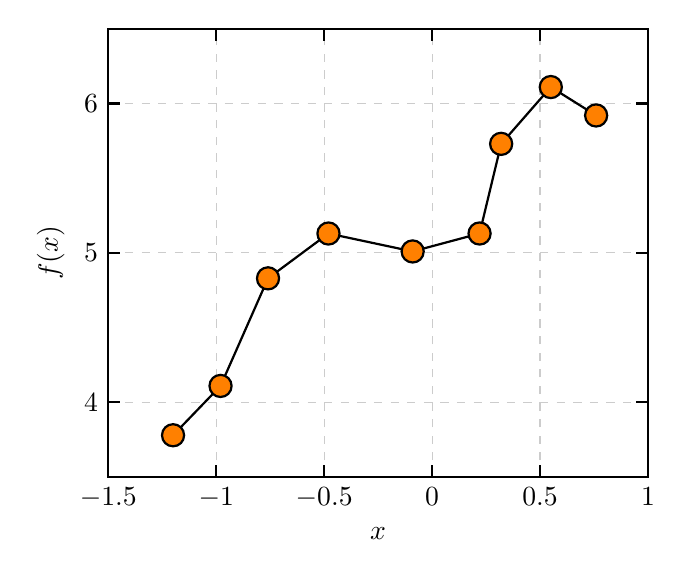
\begin{tikzpicture}
\begin{axis}[
every axis/.style={color=black, solid, thick},
xlabel = {$x$},		% подпись оси x
ylabel = {$f(x)$},	% подпись оси y
xmin=-1.5, xmax=1,
ymin=3.5, ymax=6.5,
xtick style={thick, black},
ytick style={thick, black},
grid=major,		
major grid style={color=black!20, dashed, thin},
]
\addplot[mark=*, mark size=4pt, mark options={fill=orange, draw=black, solid}] coordinates 
{(-1.2,3.78) (-0.98,4.11) (-0.76,4.83) (-0.48,5.13) (-0.09,5.01) (0.22,5.13) (0.32,5.73) (0.55,6.11) (0.76,5.92)};
\end{axis}
\end{tikzpicture}
\end{center}
% *******************************
% x1
\item
Апроксимацию функции $f(x)$ в узлах $\{x_{0}<x_{1}<x_{2}\}$
полиномом Лагранжа второго порядка $L_2(x)$, используя данные:
\begin{center}
\begin{tabular}{| l | *{4}{l}|}
\hline
$i$&0&1&2&\dots\\
\hline
$x_i$&-1,2&-0,98&-0,76&\dots\\
\hline
$f(x_i)$&3,78&4,11&4,83&\dots \\
\hline
\end{tabular}
\end{center}
\begin{gather*}
\begin{matrix}
L_2(x)&=&\dfrac{(x-(-0,98))(x-(-0,76))}{(-1,20-(-0,98))(-1,20-(-0,76))}\cdot3,78&+\\[1em]
&+&\dfrac{(x-(-1,20))(x-(-0,76))}{(-0,98-(-1,20))(-0,98-(-0,76))}\cdot4,11&+\\[1em]
&+&\dfrac{(x-(-1,20))(x-(-0,98))}{(-0,76-(-1,20))(-0,76-(-0,98))}\cdot4,83
\end{matrix}
\end{gather*}
Проводя элементарные алгебраические преобразования полином Лагранжа 
в пределах отрезка $[-1,2;-0,76]$ имеет вид:
\begin{gather*}
L_2(x)=4,028925620\cdot x^2+10,28305785\cdot x+10,31801653
\end{gather*}
% *******************************
%	График функций
%
\begin{center}
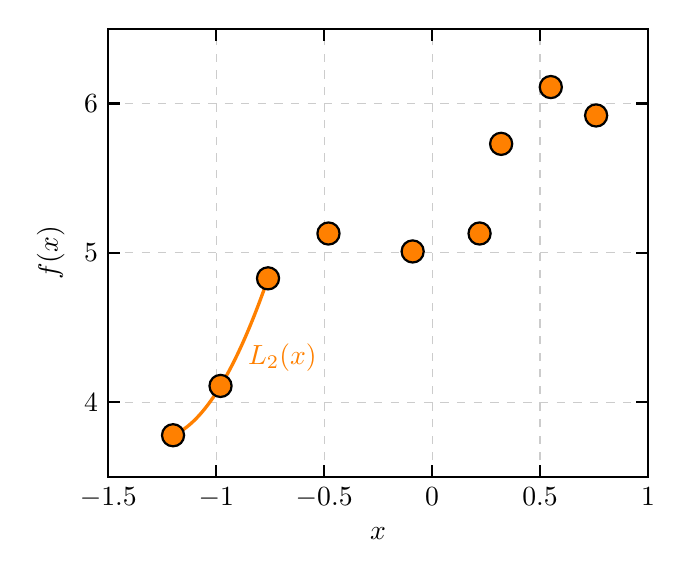
\begin{tikzpicture}
\begin{axis}[
every axis/.style={color=black, solid, thick},
xlabel = {$x$},		% подпись оси x
ylabel = {$f(x)$},	% подпись оси y
xmin=-1.5, xmax=1,
ymin=3.5, ymax=6.5,
xtick style={thick, black},
ytick style={thick, black},
grid=major,		
major grid style={color=black!20, dashed, thin},
]
\addplot[only marks, mark=*, mark size=4pt, mark options={fill=orange, draw=black, solid}] coordinates 
{(-1.2,3.78) (-0.98,4.11) (-0.76,4.83) (-0.48,5.13) (-0.09,5.01) (0.22,5.13) (0.32,5.73) (0.55,6.11) (0.76,5.92)};
\addplot[color=orange, very thick, samples=50, domain=-1.2:-0.76] {
4.028925620*x^2+10.28305785*x+10.31801653
};
\draw[color=orange] (axis cs: -0.9,4.3) node [right] {$L_2(x)$};
\end{axis}
\end{tikzpicture}
\end{center}
% *******************************
Определим первую и вторую производную функции $f(x)$ в точке $x_1=-0,98$:
\begin{gather*}
f^{\prime}(-0,98)\approx L_2^{\prime}(-0,98)=2,386363635\\
f^{\prime\prime}(-0,98)\approx L_2^{\prime\prime}(-0,98)=8,057851240
\end{gather*}

% x2
\item
Апроксимацию функции $f(x)$ в узлах $\{x_{1}<x_{2}<x_{3}\}$
полиномом Лагранжа второго порядка $L_2(x)$, используя данные:
\begin{center}
\begin{tabular}{| l | *{5}{l}|}
\hline
$i$&\dots&1&2&3&\dots\\
\hline
$x_i$&\dots&-0,98&-0,76&-0,48&\dots\\
\hline
$f(x_i)$&\dots&4,11&4,83&5,13&\dots\\
\hline
\end{tabular}
\\[1em]
\end{center}

\begin{gather*}
\begin{matrix}
L_2(x)&=&\dfrac{(x-(-0,76))(x-(-0,48))}{(-0,98-(-0,76))(-0,98-(-0,48))}\cdot4,11&+\\[1em]
&+&\dfrac{(x-(-0,98))(x-(-0,48))}{(-0,76-(-0,98))(-0,76-(-0,48))}\cdot4,83&+\\[1em]
&+&\dfrac{(x-(-0,98))(x-(-0,76))}{(-0,48-(-0,98))(-0,48-(-0,76))}\cdot5,13
\end{matrix}
\end{gather*}
Проводя элементарные алгебраические преобразования полином Лагранжа 
в пределах отрезка $[-0,98;-0,48]$ имеет вид:
\begin{gather*}
L_2(x)=-4.402597390\cdot x^2-4.387792189\cdot x+4.038218187
\end{gather*}
% *******************************
%	График функций
%
\begin{center}
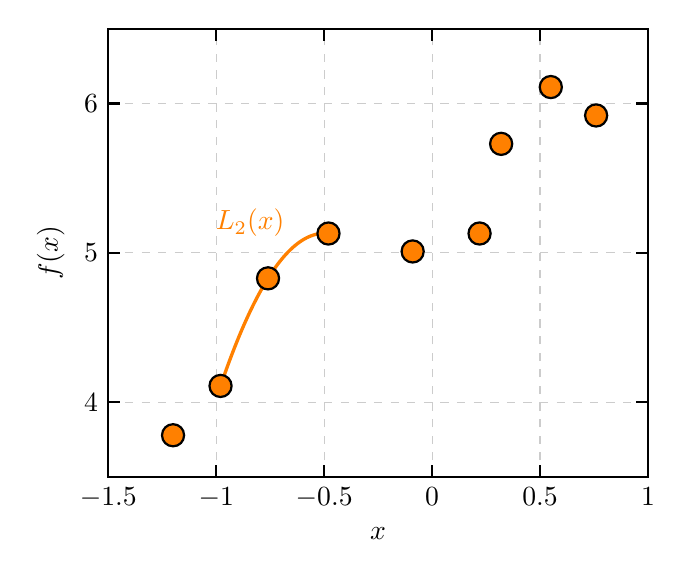
\begin{tikzpicture}
\begin{axis}[
every axis/.style={color=black, solid, thick},
xlabel = {$x$},		% подпись оси x
ylabel = {$f(x)$},	% подпись оси y
xmin=-1.5, xmax=1,
ymin=3.5, ymax=6.5,
xtick style={thick, black},
ytick style={thick, black},
grid=major,		
major grid style={color=black!20, dashed, thin},
]
\addplot[only marks, mark=*, mark size=4pt, mark options={fill=orange, draw=black, solid}] coordinates 
{(-1.2,3.78) (-0.98,4.11) (-0.76,4.83) (-0.48,5.13) (-0.09,5.01) (0.22,5.13) (0.32,5.73) (0.55,6.11) (0.76,5.92)};
\addplot[color=orange, very thick, samples=50, domain=-0.98:-0.48] {
-4.402597390*x^2-4.387792189*x+4.038218187
};
\draw[color=orange] (axis cs: -1.05,5.2) node [right] {$L_2(x)$};
\end{axis}
\end{tikzpicture}
\end{center}
% *******************************
Определим первую и вторую производную функции $f(x)$ в точке $x_2=-0,76$:
\begin{gather*}
f^{\prime}(-0,76)\approx L_2^{\prime}(-0,76)=2,304155844\\
f^{\prime\prime}(-0,76)\approx L_2^{\prime\prime}(-0,76)=-8,805194780
\end{gather*}
% x3
\item
Апроксимацию функции $f(x)$ в узлах $\{x_{2}<x_{3}<x_{4}\}$
полиномом Лагранжа второго порядка $L_2(x)$, используя данные:
\begin{center}
\begin{tabular}{| l | *{5}{l}|}
\hline
$i$&\dots&2&3&4&\dots\\
\hline
$x_i$&\dots&-0,76&-0,48&-0,09&\dots\\
\hline
$f(x_i)$&\dots&4,83&5,13&5,01&\dots\\
\hline
\end{tabular}
\\[1em]
\end{center}
\begin{gather*}
\begin{matrix}
L_2(x)&=&\dfrac{(x-(-0,48))(x-(-0,09))}{(-0,76-(-0,48))(-0,76-(-0,09))}\cdot4,83&+\\[1em]
&+&\dfrac{(x-(-0,76))(x-(-0,09))}{(-0,48-(-0,76))(-0,48-(-0,09))}\cdot5,13&+\\[1em]
&+&\dfrac{(x-(-0,76))(x-(-0,48))}{(-0,09-(-0,76))(-0,09-(-0,48))}\cdot5,01
\end{matrix}
\end{gather*}
Проводя элементарные алгебраические преобразования полином Лагранжа 
в пределах отрезка $[-0,76;-0,09]$ имеет вид:
\begin{gather*}
L_2(x)=-2.058389370\cdot x^2-1.480974249\cdot x+4.893385272
\end{gather*}
% *******************************
%	График функций
%
\begin{center}
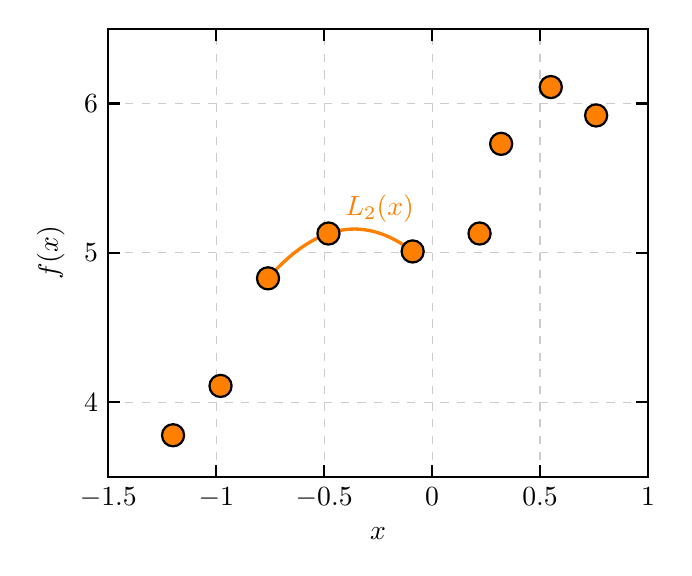
\begin{tikzpicture}
\begin{axis}[
every axis/.style={color=black, solid, thick},
xlabel = {$x$},		% подпись оси x
ylabel = {$f(x)$},	% подпись оси y
xmin=-1.5, xmax=1,
ymin=3.5, ymax=6.5,
xtick style={thick, black},
ytick style={thick, black},
grid=major,		
major grid style={color=black!20, dashed, thin},
]
\addplot[only marks, mark=*, mark size=4pt, mark options={fill=orange, draw=black, solid}] coordinates 
{(-1.2,3.78) (-0.98,4.11) (-0.76,4.83) (-0.48,5.13) (-0.09,5.01) (0.22,5.13) (0.32,5.73) (0.55,6.11) (0.76,5.92)};
\addplot[color=orange, very thick, samples=50, domain=-0.76:-0.09] {
-2.058389370*x^2-1.480974249*x+4.893385272
};
\draw[color=orange] (axis cs: -0.45,5.3) node [right] {$L_2(x)$};
\end{axis}
\end{tikzpicture}
\end{center}
% *******************************
Определим первую и вторую производную функции $f(x)$ в точке $x_3=-0,48$:
\begin{gather*}
f^{\prime}(-0,48)\approx L_2^{\prime}(-0,48)=0,495079546\\
f^{\prime\prime}(-0,48)\approx L_2^{\prime\prime}(-0,48)=-4,116778740
\end{gather*}
%x4
\item
Апроксимацию функции $f(x)$ в узлах $\{x_{3}<x_{4}<x_{5}\}$
полиномом Лагранжа второго порядка $L_2(x)$, используя данные:
\begin{center}
\begin{tabular}{| l | *{5}{l}|}
\hline
$i$&\dots&3&4&5&\dots\\
\hline
$x_i$&\dots&-0,48&-0,09&0,22&\dots\\
\hline
$f(x_i)$&\dots&5,13&5,01&5,13&\dots\\
\hline
\end{tabular}
\\[1em]
\end{center}
\begin{gather*}
\begin{matrix}
L_2(x)&=&
\dfrac{(x-(-0,09))(x-0,22)}{(-0,48-(-0,09))(-0,48-0,22)}\cdot5,13&+\\[1em]
&+&\dfrac{(x-(-0,48))(x-0,22)}{(-0,09-(-0,48))(-0,09-0,22)}\cdot5,01&+\\[1em]
&+&\dfrac{(x-(-0,48))(x-(-0,09))}{(0,22-(-0,48))(0,22-(-0,09))}\cdot5,13
\end{matrix}
\end{gather*}
Проводя элементарные алгебраические преобразования полином Лагранжа 
в пределах отрезка $[-0,48;0,22]$ имеет вид:
\begin{gather*}
L_2(x)=0,9925558300\cdot x^2+0,2580645177\cdot x+5,025186105
\end{gather*}
% *******************************
%	График функций
%
\begin{center}
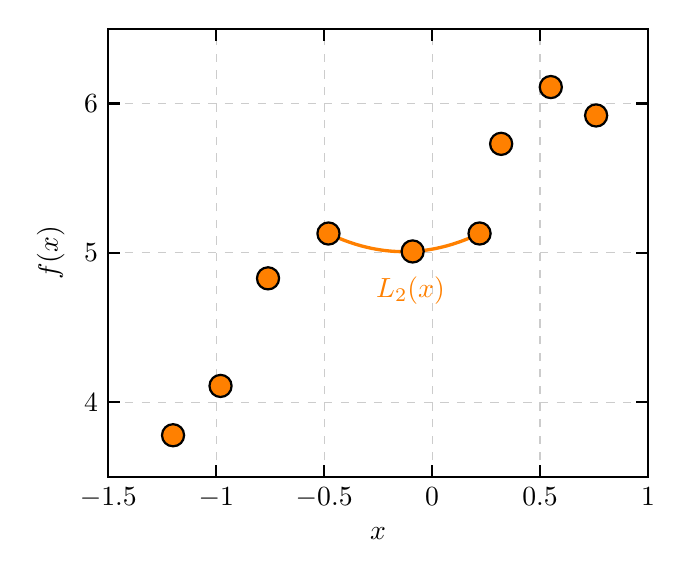
\begin{tikzpicture}
\begin{axis}[
every axis/.style={color=black, solid, thick},
xlabel = {$x$},		% подпись оси x
ylabel = {$f(x)$},	% подпись оси y
xmin=-1.5, xmax=1,
ymin=3.5, ymax=6.5,
xtick style={thick, black},
ytick style={thick, black},
grid=major,		
major grid style={color=black!20, dashed, thin},
]
\addplot[only marks, mark=*, mark size=4pt, mark options={fill=orange, draw=black, solid}] coordinates 
{(-1.2,3.78) (-0.98,4.11) (-0.76,4.83) (-0.48,5.13) (-0.09,5.01) (0.22,5.13) (0.32,5.73) (0.55,6.11) (0.76,5.92)};
\addplot[color=orange, very thick, samples=50, domain=-0.48:0.22] {
0.9925558300*x^2+0.2580645177*x+5.025186105
};
\draw[color=orange] (axis cs: -0.1,4.75) node {$L_2(x)$};
\end{axis}
\end{tikzpicture}
\end{center}
% *******************************
Определим первую и вторую производную функции $f(x)$ в точке $x_4=-0,09$:
\begin{gather*}
f^{\prime}(-0,09)\approx L_2^{\prime}(-0,09)=0,0794044683\\
f^{\prime\prime}(-0,09)\approx L_2^{\prime\prime}(-0,09)=1,985111660
\end{gather*}
%x5
\item
Апроксимацию функции $f(x)$ в узлах $\{x_{4}<x_{5}<x_{6}\}$
полиномом Лагранжа второго порядка $L_2(x)$, используя данные:
\begin{center}
\begin{tabular}{| l | *{5}{l}|}
\hline
$i$&\dots&4&5&6&\dots\\
\hline
$x_i$&\dots&-0,09&0,22&0,32&\dots\\
\hline
$f(x_i)$&\dots&5,01&5,13&5.73&\dots\\
\hline
\end{tabular}
\\[1em]
\end{center}
\begin{gather*}
\begin{matrix}
L_2(x)&=&
\dfrac{(x-0,22)(x-0,32)}{(-0,09-0,22)(-0,09-0,32)}\cdot5,01&+\\[1em]
&+&\dfrac{(x-(-0,09))(x-0,32)}{(0,22-(-0,09))(0,22-0,32)}\cdot5,13&+\\[1em]
&+&\dfrac{(x-(-0,09))(x-0,22)}{(0,32-(-0,09))(0,32-0,22)}\cdot5,73
\end{matrix}
\end{gather*}
Проводя элементарные алгебраические преобразования полином Лагранжа 
в пределах отрезка $[-0,09;0,32]$ имеет вид:
\begin{gather*}
L_2(x)=13,69000778\cdot x^2-1,392604236\cdot x+4,773776556
\end{gather*}
% *******************************
%	График функций
%
\begin{center}
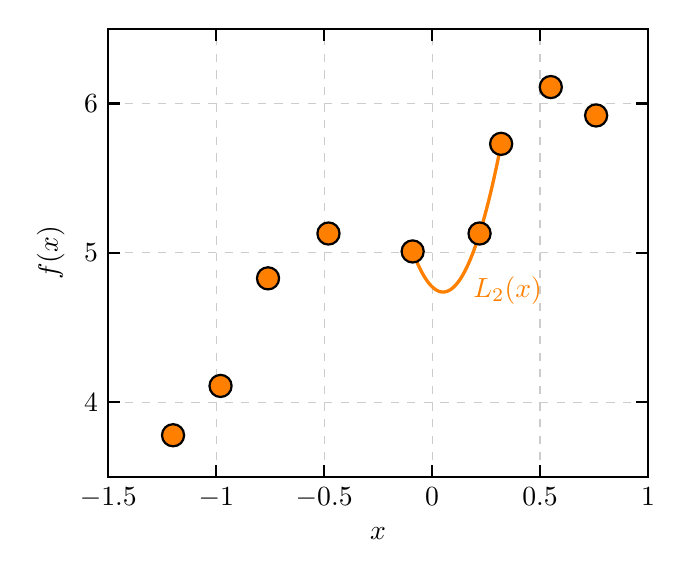
\begin{tikzpicture}
\begin{axis}[
every axis/.style={color=black, solid, thick},
xlabel = {$x$},		% подпись оси x
ylabel = {$f(x)$},	% подпись оси y
xmin=-1.5, xmax=1,
ymin=3.5, ymax=6.5,
xtick style={thick, black},
ytick style={thick, black},
grid=major,		
major grid style={color=black!20, dashed, thin},
]
\addplot[only marks, mark=*, mark size=4pt, mark options={fill=orange, draw=black, solid}] coordinates 
{(-1.2,3.78) (-0.98,4.11) (-0.76,4.83) (-0.48,5.13) (-0.09,5.01) (0.22,5.13) (0.32,5.73) (0.55,6.11) (0.76,5.92)};
\addplot[color=orange, very thick, samples=50, domain=-0.09:0.32] {
13.69000778*x^2-1.392604236*x+4.773776556
};
\draw[color=orange] (axis cs: 0.35,4.75) node {$L_2(x)$};
\end{axis}
\end{tikzpicture}
\end{center}
% *******************************
Определим первую и вторую производную функции $f(x)$ в точке $x_5=0,22$:
\begin{gather*}
f^{\prime}(0,22)\approx L_2^{\prime}(0,22)=4,630999187\\
f^{\prime\prime}(0,22)\approx L_2^{\prime\prime}(0,22)=27,38001556
\end{gather*}
%x6
\item
Апроксимацию функции $f(x)$ в узлах $\{x_{5}<x_{6}<x_{7}\}$
полиномом Лагранжа второго порядка $L_2(x)$, используя данные:
\begin{center}
\begin{tabular}{| l | *{5}{l}|}
\hline
$i$&\dots&5&6&7&\dots\\
\hline
$x_i$&\dots&0,22&0,32&0,55&\dots\\
\hline
$f(x_i)$&\dots&5,13&5.73&6,11&\dots\\
\hline
\end{tabular}
\\[1em]
\end{center}
\begin{gather*}
\begin{matrix}
L_2(x)&=&
\dfrac{(x-0,32)(x-0,55)}{(0,22-0,32)(0,22-0,55)}\cdot5,13&+\\[1em]
&+&\dfrac{(x-0,22)(x-0,55)}{(0,32-0,22)(0,32-0,55)}\cdot5,73&+\\[1em]
&+&\dfrac{(x-0,22)(x-0,32)}{(0,55-0,22)(0,55-0,32)}\cdot6,11
\end{matrix}
\end{gather*}
Проводя элементарные алгебраические преобразования полином Лагранжа 
в пределах отрезка $[0,22;0,55]$ имеет вид:
\begin{gather*}
L_2(x)=-13,17523062\cdot x^2+13,11462456\cdot x+2,882463758
\end{gather*}
% *******************************
%	График функций
%
\begin{center}
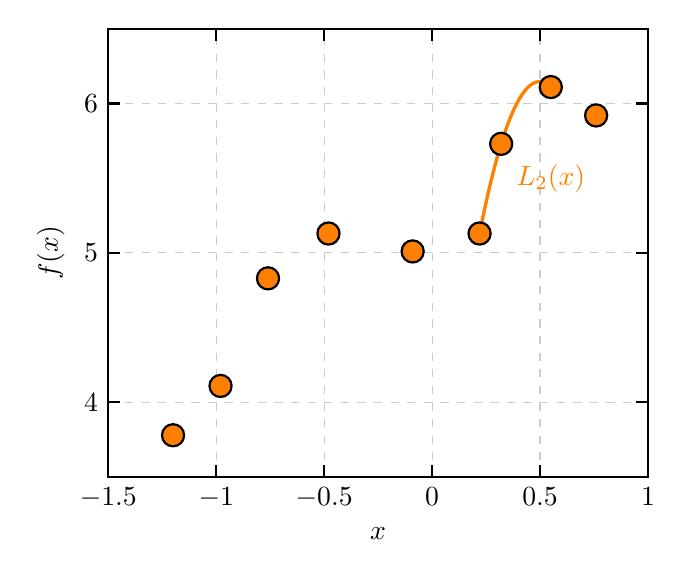
\begin{tikzpicture}
\begin{axis}[
every axis/.style={color=black, solid, thick},
xlabel = {$x$},		% подпись оси x
ylabel = {$f(x)$},	% подпись оси y
xmin=-1.5, xmax=1,
ymin=3.5, ymax=6.5,
xtick style={thick, black},
ytick style={thick, black},
grid=major,		
major grid style={color=black!20, dashed, thin},
]
\addplot[only marks, mark=*, mark size=4pt, mark options={fill=orange, draw=black, solid}] coordinates 
{(-1.2,3.78) (-0.98,4.11) (-0.76,4.83) (-0.48,5.13) (-0.09,5.01) (0.22,5.13) (0.32,5.73) (0.55,6.11) (0.76,5.92)};
\addplot[color=orange, very thick, samples=50, domain=0.22:0.55] {
-13.17523062*x^2+13.11462456*x+2.882463758
};
\draw[color=orange] (axis cs: 0.55,5.5) node {$L_2(x)$};
\end{axis}
\end{tikzpicture}
\end{center}
% *******************************
Определим первую и вторую производную функции $f(x)$ в точке $x_6=0,32$:
\begin{gather*}
f^{\prime}(0,32)\approx L_2^{\prime}(0,32)=4,682476963\\
f^{\prime\prime}(0,32)\approx L_2^{\prime\prime}(0,32)=-26,35046124
\end{gather*}
% x7
\item
Апроксимацию функции $f(x)$ в узлах $\{x_{6}<x_{7}<x_{8}\}$
полиномом Лагранжа второго порядка $L_2(x)$, используя данные:
\begin{center}
\begin{tabular}{| l | *{4}{l}|}
\hline
$i$&\dots&6&7&8\\
\hline
$x_i$&\dots&0,32&0,55&0,76\\
\hline
$f(x_i)$&\dots&5.73&6,11&5,92\\
\hline
\end{tabular}
\\[1em]
\end{center}
\begin{gather*}
\begin{matrix}
L_2(x)&=&
\dfrac{(x-0,55)(x-0,76)}{(0,32-0,55)(0,32-0,76)}\cdot5,73&+\\[1em]
&+&\dfrac{(x-0,32)(x-0,76)}{(0,55-0,32)(0,55-0,76)}\cdot6,11&+\\[1em]
&+&\dfrac{(x-0,32)(x-0,55)}{(0,76-0,32)(0,76-0,55)}\cdot5,92
\end{matrix}
\end{gather*}
Проводя элементарные алгебраические преобразования полином Лагранжа 
в пределах отрезка $[0,32;0,76]$ имеет вид:
\begin{gather*}
L_2(x)=-5,811217790\cdot x^2+6,707933391\cdot x+4,178530017
\end{gather*}
% *******************************
%	График функций
%
\begin{center}
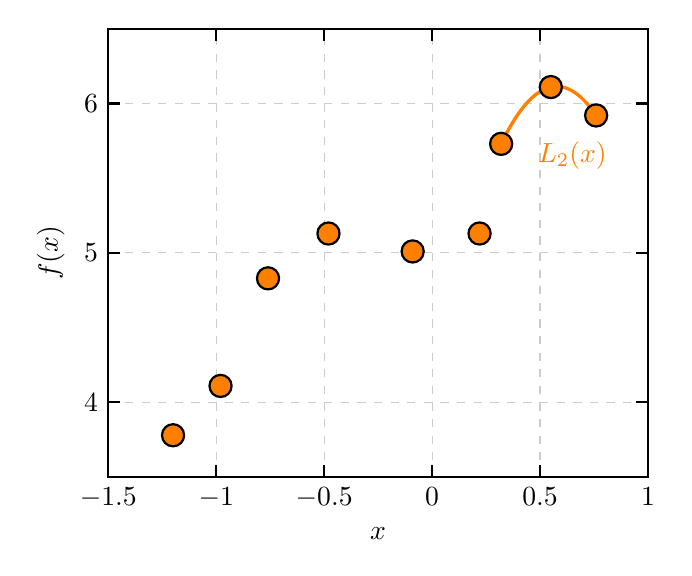
\begin{tikzpicture}
\begin{axis}[
every axis/.style={color=black, solid, thick},
xlabel = {$x$},		% подпись оси x
ylabel = {$f(x)$},	% подпись оси y
xmin=-1.5, xmax=1,
ymin=3.5, ymax=6.5,
xtick style={thick, black},
ytick style={thick, black},
grid=major,		
major grid style={color=black!20, dashed, thin},
]
\addplot[only marks, mark=*, mark size=4pt, mark options={fill=orange, draw=black, solid}] coordinates 
{(-1.2,3.78) (-0.98,4.11) (-0.76,4.83) (-0.48,5.13) (-0.09,5.01) (0.22,5.13) (0.32,5.73) (0.55,6.11) (0.76,5.92)};
\addplot[color=orange, very thick, samples=50, domain=0.32:0.76] {
-5.811217790*x^2+6.707933391*x+4.178530017
};
\draw[color=orange] (axis cs: 0.65,5.65) node {$L_2(x)$};
\end{axis}
\end{tikzpicture}
\end{center}
% *******************************
Определим первую и вторую производную функции $f(x)$ в точке $x_7=0,55$:
\begin{gather*}
f^{\prime}(0,55)\approx L_2^{\prime}(0,55)=0,315593822\\
f^{\prime\prime}(0,55)\approx L_2^{\prime\prime}(0,55)=-11,62243558
\end{gather*}
\item
Таким образом, определены значения первой $f^{\prime}(x_i)$ и
второй $f^{\prime\prime}(x_i)$ производной функции $f(x)$ 
в каждом внутреннем узле сетки $\{x_i\}$:
\begin{center}
\begin{tabular}{ l *{7}{l}}
\toprule
$x$&-0,98&-0,76&-0,48&-0,09&0,22&0,32&0,55\\
\midrule
$f^{\prime}(x)$&2,39&2,30&0,50&0,08&4,63&4,68&0,32\\
\midrule
$f^{\prime\prime}(x)$&8,06&-8,81&-4,12&1,99&27,38&-26,35&-11,62\\
\bottomrule
\end{tabular} 
\end{center}
% *******************************
%	График функций
%
\begin{center}
\begin{tikzpicture}[background rectangle/.style={fill=olive!10}, show background rectangle]
\begin{axis}[
every axis/.style={color=black, solid, thick},
xlabel = {$x$},		% подпись оси x
ylabel = {$\textcolor{blue}{f^{\prime}(x)}$},	% подпись оси y
xmin=-1.5, xmax=1,
ymin=-0.5, ymax=5,
xtick style={thick, black},
ytick style={thick, black},
grid=major,		
major grid style={color=black!20, dashed, thin},
]
\addplot[blue,mark=*, mark size=4pt, mark options={fill=blue!50, draw=black, solid}] coordinates 
{(-0.98,2.39) (-0.76,2.30) (-0.48,0.50) (-0.09,0.08) (0.22,4.63) (0.32,4.68) (0.55,0.32)};
\end{axis}
\end{tikzpicture}
\begin{tikzpicture}[background rectangle/.style={fill=olive!10}, show background rectangle]
\begin{axis}[
every axis/.style={color=black, solid, thick},
xlabel = {$x$},		% подпись оси x
ylabel = {$\textcolor{red}{f^{\prime\prime}(x)}$},	% подпись оси y
xmin=-1.5, xmax=1,
ymin=-30, ymax=30,
xtick style={thick, black},
ytick style={thick, black},
grid=major,		
major grid style={color=black!20, dashed, thin},
]
\addplot[red,mark=*, mark size=4pt, mark options={fill=red!75, draw=black, solid}] coordinates 
{(-0.98,8.06) (-0.76,-8.81) (-0.48,-4.12) (-0.09,1.99) (0.22,27.38) (0.32,-26.35) (0.55,-11.62)};
\end{axis}
\end{tikzpicture}
\end{center}

\end{enumerate}

%\end{document}